
%%%%%%%%%%%%%%%%%%%%%%% file typeinst.tex %%%%%%%%%%%%%%%%%%%%%%%%%
%
% This is the LaTeX source for the instructions to authors using
% the LaTeX document class 'llncs.cls' for contributions to
% the Lecture Notes in Computer Sciences series.
% http://www.springer.com/lncs       Springer Heidelberg 2006/05/04
%
% It may be used as a template for your own input - copy it
% to a new file with a new name and use it as the basis
% for your article.
%
% NB: the document class 'llncs' has its own and detailed documentation, see
% ftp://ftp.springer.de/data/pubftp/pub/tex/latex/llncs/latex2e/llncsdoc.pdf
%
%%%%%%%%%%%%%%%%%%%%%%%%%%%%%%%%%%%%%%%%%%%%%%%%%%%%%%%%%%%%%%%%%%%


\documentclass[runningheads,a4paper]{llncs}

\usepackage{amssymb}
\setcounter{tocdepth}{3}
\usepackage{graphicx}

\usepackage{url}
\urldef{\mailsa}\path|{alfred.hofmann, ursula.barth, ingrid.haas, frank.holzwarth,|
\urldef{\mailsb}\path|anna.kramer, leonie.kunz, christine.reiss, nicole.sator,|
\urldef{\mailsc}\path|erika.siebert-cole, peter.strasser, lncs}@springer.com|
\newcommand{\keywords}[1]{\par\addvspace\baselineskip
\noindent\keywordname\enspace\ignorespaces#1}

\usepackage{todonotes}
\newcommand{\yongli}{\todo[author=YL,color=green,inline]}
\newcommand{\naoki}{\todo[author=NK,color=yellow,inline]}
\begin{document}

\mainmatter  % start of an individual contribution

% first the title is needed
\title{Change Detection From Media Sharing Community }

% the name(s) of the author(s) follow(s) next
%
% NB: Chinese authors should write their first names(s) in front of
% their surnames. This ensures that the names appear correctly in
% the running heads and the author index.
%

\author{Naoki Kito
\and Dr.Xiangmin Zhou\and Assoc Prof. James Thom}

\maketitle


\begin{abstract}
From ancient time, the damages or the destructions to the countries caused by the natural disasters were the major issues. Recently, through the improvement of image change detection technologies, social media and the high-resolution images, the damages caused by natural disasters can be analysed in more details to identify the situations in the cities or towns. Many researchers approached to analyse the damage by using the aerial images and the satellites images, but these images are often published to the public after the things settle down. However, when the disasters happen, people want the information of disasters as soon as possible. This research proposes to investigate how the social media images and the image change detection techniques can be used to identify the damages caused by the natural disasters. We first propose a framework that takes advantages of fast clustering and image near duplicate identification for the change detection in disasters. Then we model the social images by exploiting the image tags and location information. Following that, we propose a recursive 2 means algorithm over the new data model. Finally, we refine the changes by local interest point-based similarity matching. Extensive experiments have been done to evaluate the high effectiveness and efficiency of our approach.
\end{abstract}


\section{Introduction}

Before, during and after the natural disasters, 
information about the damages and the current situations are vital for people to make decisions for their next actions. 
For example, 
the Nepal earthquake in 2015 did a huge damage to everything, including buildings, roads, infrastructure, and people, which resulted in 8,019 people died and 17,866 people injured; 
in a Tokyo earthquake, people are still able to walk back home since the earthquake damage the infrastructure, but not the buildings and paths. 
A recent study \cite{110009470680} found that people would like to know earthquake size and epicentre. 
Moreover, knowing these information could prevent the secondary and tertiary disasters. 
It is also found that in Tokyo, only 67.8\% of people managed to get back their house on the day of an earthquake,
and the rest 32.2\% had to become ``\emph{homeless}", among them 2\% failed to going back home only because they could not find the safe path. 
People want the information about earthquakes, but there is always the question ``How should the people get the information of earthquakes?". 

Recently, there are lots of researchers had approached to detect the damages caused by the natural disasters by using the change detection techniques with the aerial images. However, the aerial images consume longer times retrieve and harder to get compare to the other images.
On the other hand, social media is pervasive, and updates very quickly especially on large events, e.g. natural disasters, by millions of people all the time. 
Thus, we investigate the problem of change detection from social media images, so as to let the public aware of the latest situations of natural disasters on the spot. 
One of the challenges here is the large-scale of the social media images,
which makes current change detection techniques infeasible if not impossible. 
One of the limitation of using the large-scale images with current change detection techniques is the time cost. 
\yongli{Explain why time cost is a issue for them?}
Another limitation is the unstable/unrelated images. 
The social media image features are made by the up-loader and 
this human inputs make the unstable/unrelated images. 
\yongli{are we solving this?}
The image rotation, resolution and the quality of the images also the concern of the limitation.

%In this research, we target to detect the damages to the infrastructures and buildings, and this project investigates image change detection techniques and the social media images. 

%In order to successfully support these tasks, the images from the social media have to cluster with the proper groups to make sure the gathered images are relevant to the natural disasters. Furthermore, the change detection system should be able to detect the damages of buildings and the roads.

%Our approach is to find the relevant images from the social media will be the Social Media Image Similarity, which is the combination of the Jaccard Similarity and the Location Similarity. Then, the images will be clustered by the Recursive 2-Means  algorithm \cite{1017616}. Finally, we are using a PCA-SIFT algorithm to match the before and the after images and find the changes between the images.
%In this paper, there are three alternative approaches to solve the questions. Firstly, the Jaccard Keywords Similarity \cite{Jaccard} is used to find the similarity between the user inputs and the tags(image tags, titles/topics and time) on the social media images. This will group or limit the images to a certain extent. Secondly, the Location Distance Similarity makes the groups of images more relevant to the natural disasters, by determine the location of the disaster happens.
%At the end of the clustering, it uses the PCA-SIFT to match before and after the disaster images.

To solve the limitations, 
we deploy existing clustering technique before using the change detection methods to detect the changes. 
By applying the clustering methods to the large-scale image datasets, 
we are able to retrieve the related images from the clustered images for the change detection. 
Only applying the change detection method to the related images should increase the time performance and the accuracy of the change detection.
We use the Recursive 2 Means clustering and the new feature, Social Image Similarity is proposed for the data sets of the clustering.  The SIS is the total similarity between the images and it is the combination of the Tags Jaccard Similarity and the Locations Similarity.
The tags are the texture data which present what the images contain and the locations are the place where the images are upload to the social media.
Finally, we are using the PCA-SIFT algorithm to find the image similarities.

\yongli{It is still too detailed. I think a highlevel summarization about your technique would be better. After that, maybe one/two sentences for the details, but not too detailed.}

The contributions of this study are as follows:
\begin{itemize}
\item New Feature Social Image Similarity
\item Weighted Tags 
\item ...
\end{itemize}
\yongli{Please list the contributions here}

The rest of the paper is structured as follows:
Section~\ref{sec-bg} reviews the related work;
Section~\ref{sec-framework} presents the framework proposed in this study;
Section~\ref{sec-datamodelling} details the modelling of the social media data;
Section~\ref{sec-algorithm} presents the proposed change detection algorithm;
Section~\ref{sec-evaluation} includes the experiment evaluation;
Section~\ref{sec-con} concludes the paper. 

\section{Related Work}\label{sec-bg}
 Lu et al., 2004\cite{lu2004change} state that there are seven categories for the change detection algorithms, which are: 1.Algebra 2.Transformation 3.Classification 4.Advance models 5.Geographical Information System (GIS) approaches 6.visual analysis  7.Other. \cite{lu2004change}. Lu et al.,2004 \cite{lu2004change} also state that these algorithms have their own unique characteristic, advantages, and disadvantages. 
These various change detections are commonly used in remote sensing, which often use to find the changes of the land surface, nature, and cities/towns. For another example, change detection in video surveillance often uses for the security purpose.

\subsection{K-Means}

The Recursive 2 Means algorithm are used. 
After the clustering, the PCA-SIFT is used to find the changes between the before and the after images as shown in figure \ref{fig:Frame}.
The Recursive 2 means Clustering has the similar process with the standard K-MEAN Algorithm, but instead of having several K clusters(more than 2), the Recursive 2 means clustering only has two clusters for each layer\footnotemark.\\
The Recursive 2 means clustering steps:

\begin{itemize}
\item 1: Create 2 random centroids(can be pre-made)
\item 2: For each N, find the closest centroid and assign N to the K
\item 3: Update the K centroids to the average of current assign N
\item 4: Repeat the 2 and 3 until the K stop moving
\item 5: Repeat 1 to 4 within the clustered data
\end{itemize}

\footnotetext[3]{One of the type of Hash Index in Java programming}

\begin{figure}[h]
	\centering
	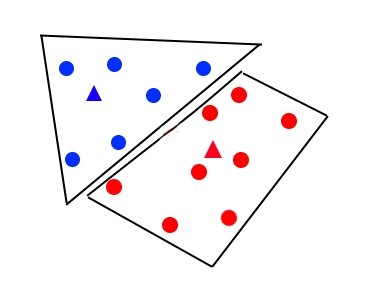
\includegraphics[width=4cm,bb=0 0 377 300]{Sample2mean1.jpg}
	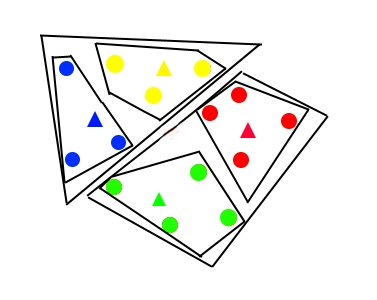
\includegraphics[width=4cm,bb=0 0 377 300]{Sample2mean2.jpg}	
	\caption{Recursive 2 Means Cluster Sample process}\label{fig:2MEANS}
	{\footnotesize The left figure shows the first cluster(step 1 to 4) result. The right figure shows the second clustering process(step 5). }
\end{figure}

As figure \ref{fig:2MEANS} shows, the Recursive 2 means cluster will always keep the number of K(cluster) to 2 for each layer. However, the number of total K(clusters) at the end of the process will have more than 2. For example, there are 4 clusters in figure \ref{fig:2MEANS}. 
In H Gifford \cite{giffordhierarchical} experiment, it shows that the Recursive K-Means is around 10 times faster than the standard K-Means algorithm. However, Kohei et al., 2007 \cite{arai2007hierarchical} had done several k-means algorithms experiments, which were using the real world data sets and they found that the Hierarchical K-Means Algorithm's error rate was higher compared to the K-Means Algorithm, which was using CCIA(``Cluster Center Initialization Algorithm" proposed by Shehroz et al., 2004 \cite{khan2004cluster} ) for the Wine data set. They stated that this because the raw data had the far difference scales, and the error rate reduced after the normalization. They conclude that the Hierarchical K-Means has the speed benefit compared to other k-means algorithms. 

\subsection{PCA-SIFT} 
\yongli{This belongs to related work. }
After the SIFT algorithm proposed by Lowe., 1999 \cite{790410}, several image change detection algorithms developed based on the SIFT algorithm. For example,  Speeded Up Robust Features(SURF)\cite{bay2006surf} and PCA-SIFT\cite{1315206} is one of the improved version of the SIFT algorithm. Juan et al.,2009\cite{juan2009comparison} had done the performance experiment for SIFT, PCA-SIFT, and SURF. They evaluated the three algorithms based on the ``time",``scale",``Rotation",``Blue",``Illumination" and ``Affine". In their experiments, it shows that the PCA-SIFT didn't have any standout performance. However, when they summarise all of the results, even though the PCA-SIFT did not have the best performance in each experiment, it has the stable performance in all situations. Which made Juan et al.,2009\cite{juan2009comparison} to conclude that the PCA-SIFT has the best performance in overall. Therefore, in this thesis, PCA-SIFT is chosen to be the main change detection algorithm.\\
The PCA-SIFT algorithm was proposed by Yan et al.,2004\cite{1315206} and it is a combination of two algorithms ``PCA" and ``SIFT".


\subsubsection{Principal  Component  Analysis(PCA)}
The Principal  Component  Analysis(PCA) was introduced by Pearson in 1901 and developed by Hotelling 1933. In 2002, Ian, 2002 \cite{jolliffe2002principal} published the second edition book, which talked about the PCA. In the book, it mentions that the main purpose of PCA is to reduce the dimensionality of the large datasets, and identify the uncorrelated variables ``Principle Component". This dimensionality reduction has the advantages of multicollinearity and data sets visualisation. \\


\subsubsection{SIFT}
In 1999, Lowe, 1999 \cite{790410} invented SIFT algorithm and it widely used to find the similarity between the images. Lowe, 1999 \cite{790410} approached to make the local feature vectors, which were invariant to the image translation, scaling, and rotation. Vectors were also partially invariant to some other changes. There are four main approaches to make these invariant feature vectors for the images. In Lowe, 2004 \cite{Lowe2004} paper, there are 4 approaches for the SIFT:

\begin{itemize}
\item Scale-space peak selection
\item Keypoint localization
\item Orientation assignment
\item Keypoint descriptor
\end{itemize}


\section{Framework}\label{sec-framework}

In this section,
we first define two terms, \emph{change} and \emph{change detection}; 
then presents the overview of the change detection framework from social media images. 

\begin{definition}\label{def-change}
In image processing, \emph{change} is defined as the difference between the two pixels or the objects in the different images. 
Note, the \emph{difference} varies in different situations. 
In this paper, the \emph{difference} is limited to the damages to the buildings, the roads or the infrastructures, which caused by the natural disasters. Such as, when the earthquake happens and a bridge breaks down, the damage to the bridge will be the \emph{change} in this situation.  
\end{definition}

\begin{definition}
\emph{Detection} is defined as \emph{Find}.
As defined in Definition~\ref{def-change}, \emph{change} refers to the damages to the buildings, roads and infrastructures.
Thus, \emph{change detection} is defined as ``Finding the damages which cause by the earthquake or natural disasters".
\end{definition}

As shown in the Fig.~\ref{fig:Frame},
the framework includes the following two component:
\begin{itemize}
\item {\bf Retrieving relevant Images} The proposed change detection framework accepts a set of tags as input,
which are used to retrieve images from the social media community (e.g. Flickr).
While the images are retrieving, the images are separated into the before and the after natural disasters.
\item {\bf Data Modelling} The information about retrieved images include the photo ID, tags, and location features.
Firstly, we model them to numeric data, then deploy two metrics to measure the similarity between tags and locations, separately. 
Finally we fuse these two similarities to obtain the final similarity between two social images, which is terms \emph{Social Image Similarity} here. 
Then, the recursive 2 means algorithm is applied to cluster similar images into groups,
which significantly reduce the complexity of the problem of change detection based on large-scale social images. 
This will be detailed in Section~\ref{sec-datamodelling}. 
\item {\bf Detecting Changes} After the similar images are grouped together, a PCA-SIFT algorithm is applied here to find the similarities between the before and the after images and detect the damages caused by the natural disasters. 
\end{itemize}

\begin{figure}[h]
	\centering
		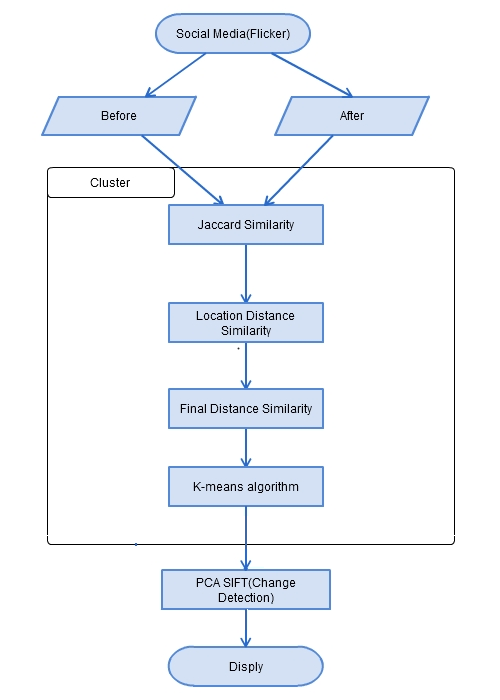
\includegraphics[width=5cm]{frame.png}	
\caption{The Framework} \label{fig:Frame}
\end{figure}

\section{Data modelling} \label{sec-datamodelling}

%As shown in the figure \ref{fig:Frame} cluster section, it uses the K-mean(Recursive 2 mean) algorithm at the end of the clustering process. Before the Recursive 2 Means process in the system, there are three processes are run to model the image features to the numeric data. These transformed data are used in the Recursive 2 Means algorithm to calculate the centre points or the centroids for the each cluster. 
In this section, we present how to model images' tags and location data for the purposed of change detection from social media images. 
Specifically, we model them to numeric data first, then measure tags and locations by using two different similarity metrics, respectively. Finally, we fuse them together to obtain the \emph{difference} of social media images. 

%Two existing algorithms are used to model the image features and the modelled data are called \textit{Distance Similarity} in this paper. By using the existing algorithms, we success to produce three distance similarities within the images. The three distance similarities are: \textit{Jaccard Distance Similarity}, \textit{Location Distance Similarity} and \textit{Social Image Similarity}. The \textit{Jaccard Distance Similarity} calculates the tags similarities with the Jaccard algorithm and the result will be range from 0 to 1. The \textit{Location Distance Similarity} calculates the geometric distances between the images. Some of the location distance similarity results contain a large number and this reduces the accuracy of clustering, so the results will be normalized.  These results are also in the range from 0 to 1. Finally, the \textit{Social Image Similarity} calculates the total distances similarity between the images. It uses the Jaccard and Location distance similarities to get the result. The Recursive 2 Means algorithm used this Distance Similarity as the data sets.

\subsection{Tag-based Similarity}
In social media, the posted images normally have some tags on it, 
which contain semantic meanings of the images. 
The tags are attached to the images by the uploaders and they may vary. 
We first weight the tags on images and then deploy a weighted version of Jaccard metric to measure the similarity between images. 
Specifically, 
the tags assign with the value of 1 as a default, but when the centroids are calculated, the tags weight will be the average of the tags appear in the images. 
We will discuss in more details about the weighted tags in section 5. 
\yongli{I suggest to explain the weights here clearly, as it is very relevant here. In addition, it is your contribution, and should be emphasised as early as possible. }
The basic equation for Jaccard Similarity from \cite{Jaccard} is: 
\yongli{can you provide a weighted version of Jaccard by using your weighted tags? this is something interesting, not the standard Jaccard equation. }
\begin{equation}\label{eq:JAAAAC}
S_{tag} = ...
\end{equation} 
\begin{equation}\label{eq:JAAAAC}
 J(A,B) = \frac{|A\cap B|}{|A\cup B|} = \frac{|A\cap B|}{|A|+|B|-|A\cap B|}
\end{equation} 

In equation \ref{eq:JAAAAC}, the `A' is the user input and the `B' is the tags. This equation calculates the distances between the user inputs and all the images tags. After the distance calculation, the average of the \textit{JDS} is calculated to find the centroid \textit{JDS}.

\begin{equation}
0< J(A,B) <1 : 0 = not match, 1 = match 
\end{equation} 
Examples: 

\begin{itemize}
\item User Input = ``Happy", ``cake"
\item Tags = ``Happy", ``fire",``rain",``party",``apple",``cake"
\end{itemize}

\begin{eqnarray}
 J(A,B) = \frac{|A\cap B|}{|A\cup B|} = \frac{|A\cap B|}{|A|+|B|-|A\cap B|} \\ = \frac{2}{|2|+|6|-|2|} = \frac{2}{6} = 0.33
\end{eqnarray} 

The equation 4 is the example of two user inputs and six image tags, and both two inputs matched with the tags. In this case, the result is `0.33', which means the image is partially related to what the user want. 
However, only using the Jaccard Similarity distances will cause the human error issues when the k-means algorithm use them as the data sets. This because the image tags could contain the unrelated tags. For example, the image of the car is tagged with the building. Therefore, to increase the accuracy of clustering we use the Location Distance Similarity.
\footnotetext{http://bit.ly/1XdoJ36}
\footnotetext[2]{http://bit.ly/1Uka1Fa}

\subsection{Location-based similarity(LDS)} 

To detect changes from images, it is important to prevent gathering the different location images, but having the similar tags.
Thus, location information is a necessary. 

%The second step is to define the location distances between the images. This will prevent gathering the different location images, but having the similar tags. The equation below is the sample location distance formula, where `D' represent the distance between the images.
%
%The distance between two images is defined as:
%\begin{equation}
%D = L2(location 2) - L1(Location 1)
%\end{equation} 
%where $D$ denotes the distance, $L1$ and $L2$ are the locations
%
%When the `D' is small or 0, this means the two images' locations are near. On the other hand, the larger number represent the images took at the different places.\\

We deploy the ``Great Circle Distance(GCD)" to calculate the distance between the images. 
The Haversine Formula \cite{10.2307/2309088} is used to calculate GCD.
However at this point, the bearing and the midpoint where not important values for the Location similarity, so it only calculates the distance between 2 points.
\begin{eqnarray}
	a = sin²(ΔLat/2) + cos Lat1 ⋅ cos Lat2 ⋅ sin²(ΔLon/2)\\
	c = 2 ⋅ atan2(  \sqrt{a},  \sqrt{(1-a)} )\\
	d = R ⋅ c 
\end{eqnarray}
Where $a$ denotes the Haversine, $c$ denotes the great circle distance in radians and  $d$ denotes the location distance.
The Haversine is using 3 points/locations to calculate the Great Circle Distance, and the above formula is using the earth's radian for the third point.
As suggested by Johor et al. 2013~\cite{Standardization},
the location distances are normalised to removed the potential biases among different features. 
Specifically, 
Johor et al. 2013 \cite{Standardization} found the `` Min-Max" standardization had the best/lowest error rate to $k$-means algorithms. 
Thus, we choose to use the ``Min-Max" as a normalization technique:
\begin{equation}
D' = \frac{D-min(D)}{max(D)-min(D)}
\end{equation} 	
where $D$ denotes the calculate location between images.
%Formula from Johor et al., 2013 \cite{Standardization}, In this formula `x' is representing the location distance. ``min(x)" and ``max(x)" is the shortest and farthest distances in the distance list.


\subsection{Social Similarity (SocSim) }

We finally define the similarity between two social images by fusing the tag-based distance and location-based distance,
which is termed as \emph{Social Similarity} (SocSim):
\begin{equation}
S_{SocSim} = \frac{1}{D+1} * S_{tag},
\end{equation} 	
where $D$ is the location-based distance and $S_{tag}$ is the tag-based similarity.
The $S_{SocSim}$ will be the range from 0 to 1. 
A larger value means the images closer to each other.

\section{Change Detection Over Large Data Sets}\label{sec-algorithm}

In this section,
we present the change detection algorithm from the large-scale social media images. 

%Since there are large data sets can be retrieved from the social media, there are two approaches to improving our clustering performance in both speed and accuracy.

\subsection{Clustering Techniques and Improvement}

The idea of the clustering algorithms is to group the large datasets into the smaller groups. Always the data within the same group have the similar data than the data in other clusters. 
The clustering allows the system to use the centroids as the references of the cluster, and by referencing the centroids the system does not have to analyse all the data in the data sets. By knowing which cluster should be analysed, it increases the speed performance. However, there are some issues or limits on the clustering methods, such as the clustering methods could not handle some attribute types, time complexity and etc \cite{Berkhin2006}. 

Moreover, Cheung~\cite{Cheung20032883} found there are 3 drawbacks for the K-MEANS algorithm. One of the drawbacks is that when the initialized(random) point are far away from the other points, it will remove immediately without learning within the learning process\footnotemark[2]. This means if the centroid is far from most of the points, the centroid's dimension is different from the major points' dimensions. In this research, there is one approach done with using this learning attitude. The approach is to pre-make the second centroid at the farthest point from the first centroid. The steps are followed by initialize the first random centroid, calculate the distance between the centroid and the points, and choose the farthest point as the second centroid. This approach is done to reduce the cycle of learning process(updating centroids) so that the process will improve the speed performance. This can be done in this research because, the main purpose of using Recursive 2 MEANS algorithm is to find the related images in the data sets and remove the unrelated images.

\footnotetext{Layer is the complete learning processes(step 1-5) for the K-MEANS}
\footnotetext[2]{The process at updating the centroid(step 2-3)}

\yongli{I suggest to move all Recursive 2 means related stuff to Section 2, as this is not your contribution. And focus on the Hash index one, and emphasis why it works, and how it works, and how much improvement it achieves, while you are using it with the k-means method.}

%The traditional methods are categorised in two categorise, the \textit{Hierarchical clustering} and the \textit{Partitioning clustering}. The \textit{Hierarchical Clustering} combines the data into clusters. It has two types top-down and bottom-up. the advantage is this can be use in any attribute types.

%The \textit{partitioning clustering method} is learning the clustering directly. k-mean is one of the type. it produce N points and use them as the center point. the data will learn base on these center points. the advantage is it does not depend on the data ordering. This reduce the time cost for sorting the data. 

The approach is to use a Hash Index technique to improve the data accessing speed. 
In the social media images often there are more than 10 tags on each image and comparing these tags between the images one by one are time-consuming.
To reduce the time expenses on tags comparison, we used the \textit{djb2} hash function techniques. The \textit{djb2} is known as best hash function technique for the string data compares to other hash function. In \textit{djb2} the hash values are populated by \textit{hash*33 + c}, where the hash is the long data and c is the string character. Daniel J. Bernstein uses the magic number 33 to times the hash data, however, he did not explain why it works better than any other constants.    
In our system, the \textit{djb2} is applied to all the images tags and the hash value is created for each tag. These hash values are used when the Jaccard Distance Similarity is calculated. The first step is making the tags on the ImageA and the ImageB to the hash values, and then it compares the ImageA hash values with ImageB hash values. Secondly, if the ImageA hash value does not exist in the ImageB hash value, it considers as a not match. So that the system does not need to compare all the tags values in the string. This hashing reduce the total number of String comparison in the Jaccard Distance Similarity.

\subsection{Using PCA-SIFT}

%In this section, the PCA-SIFT is not tested, but Yan et al., 2004 \cite{1315206} experimented and got the results, which showed that the PCA-SIFT had better performance in both accuracy and speed.

In this research, PCA-SIFT will use for two processes. Firstly, it will find the similarity between the objects. 
The main objects are the buildings, statues and other objects which are not moving. Also, the unrelated images choose by the PCA-SIFT algorithm will remove. 
The removing occur when the images have the Final Distance same or close, but the images are not what the user want.
Those removed images are used to calculate the error rates.
The second process is to detect the changes between the images if the images contain the similar objects. These process will be explained in detail at the ``Experiment" section.
\yongli{Please detail the two runs of PCA-SIFT, which is your work. ;)}


\subsection{Datasets Issues and approaches}

As mentioned in Section 4, 
the Recursive 2 MEANS algorithm uses the numeric data. So, the image features are modelled to numeric to measure the similarities between images.
However, the modelled data do not show the tags information and locations information
which causes a difficulty when the PCA-SIFT try to find the before and after images. 
Therefore, it is needed to find the tags and the weighted tags in the centroids to see the texture differences between the centroids and the distances. 
The tags in the centroids are the average of the tags within a cluster, which can be calculated with:
\begin{eqnarray}
CentroidKeyword = K_1(\frac{P_0+P_1..P_n}{n}),K_2(\frac{P_0+P_1..P_n}{n}) ...K_n(\frac{P_n}{n}),
\end{eqnarray}
where $P_n$ denotes the points, $K_n$ are the keywords and $n$ denotes the number of modelled data. If all the points in the cluster have the same keyword, the Keyword weight will be assign to 1. 
\yongli{what does 'the data' refer to?}
For example, assume there are 2 points where the point 1 contains 3 keywords and point 2 contain 5 keywords.\\
Point 1 Keywords = \{``earthquake",``apple",``happy"\}\\
Point 2 Keywords = \{``earthquake",``natural",``disaster",``apple",``Nepal"\}

\begin{eqnarray}\label{eq:pareto mle2}
&CentroidKeyword = earthqauake(\frac{P_1+P_2}{2}), apple(\frac{P_1+P_2}{2}),natural(\frac{P_1}{2}), \nonumber\\ &disaster(\frac{P_1}{2}), Nepal(\frac{P_1}{2})= earthqauake(\frac{1+1}{2}), apple(\frac{1+1}{2}), \nonumber\\
&natural(\frac{1}{2}),disaster(\frac{1}{2}),Nepal(\frac{1}{2}) .
\end{eqnarray}
\yongli{This equation is confusing. what is $V$?}
For the above sample, the centroid between two points is
\begin{displaymath}
CentroidKeyword = earthquake(1), apple(1), natural(0.5), disaster(0.5), Nepal(0.5).
\end{displaymath}
 By finding the centroid tags, we are able to know the main tags tagged within the cluster.
Comparing the before and after images clusters with the weighted centroids tags, we are able to reduce the searching loop for before and after image clusters. 
The figure 3, is the sample from the change detection application.

\begin{figure}[h]
	\centering
	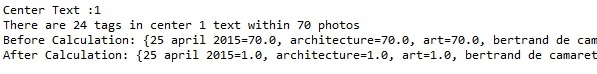
\includegraphics[width=50cm,bb=0 0 1820 73]{centroid.jpg}
	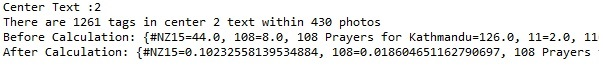
\includegraphics[width=50cm,bb=0 0 1820 73]{centroid2.jpg}
	\caption{Centroids Keywords from the appreciation}
	{\footnotesize Sample clusters tags data and weighted tags from application. Where the \textit{Center Text :1} is the first cluster and \textit{Center Text :2} is the second cluster. The line \textit{Before Calculation} and \textit{After Calculation} show the before and after the average calculation.}
\end{figure}

\pagebreak


\section{Evaluation} \label{sec-evaluation}
\subsection{Experimental set up}
\subsection{methodology}
\subsection{Effective}
\subsubsection{Effect of number tags : Effect of T}
\subsubsection{Effect of Cluster : Effect of K}
\subsubsection{comparison of EoT and EoK}
\subsection{Efficiency}
\subsubsection{Clustering with and without HASH}
\subsubsection{Data size comparison}
\subsubsection{Recursive 2 Means and K-Means}

\section{Conclusion}\label{sec-con}
\bibliographystyle{ieeetr}
% there are various bibliography styles you can set

\bibliography{reference}
% this tells latex to generate the reference list, using the references.bib file of references.
% you will need to do pdflatex <tex filename>; then bibtex <tex filename without extension>;
% pdflatex <tex filename> again twice. then you have a formatted pdf.

\end{document}

